\documentclass[11pt,a4paper]{article}
\usepackage[indonesian]{babel}
\usepackage[utf8]{inputenc}
\usepackage{geometry}
\usepackage{graphicx}
\usepackage{amsmath}
\usepackage{listings}
\usepackage{xcolor}
\usepackage{hyperref}
\usepackage{mathptmx}

\geometry{margin=2cm}

\lstset{
    basicstyle=\ttfamily\footnotesize,
    backgroundcolor=\color{gray!10},
    frame=single,
    breaklines=true,
    columns=fullflexible,
    keepspaces=true
}

\title{\textbf{Laporan Implementasi Transformer dari Nol dengan NumPy}}
\author{
    Yitzhak Edmund Tio Manalu \\
    22/499769/TK/54763 \\
    Teknologi Informasi UGM 2025
}
\date{}

\begin{document}

\maketitle

\section{Desain Arsitektur}

Implementasi ini menggunakan arsitektur \textit{decoder-only Transformer} yang mengadopsi gaya GPT (\textit{Generative Pre-trained Transformer}). Arsitektur dirancang secara modular dengan memisahkan setiap komponen ke dalam kelas atau fungsi tersendiri untuk memudahkan pemahaman dan pengujian. Pada dasarnya, model ini memproses urutan token input melalui beberapa tahapan transformasi hingga menghasilkan distribusi probabilitas untuk prediksi token berikutnya.

Tahap pertama adalah mengonversi token diskrit menjadi representasi vektor kontinu melalui \textit{token embedding}. Embedding matrix berukuran $vocab\_size \times d_{model}$ dipelajari dan hasilnya di-scale dengan faktor $\sqrt{d_{model}}$ untuk menjaga stabilitas gradien seperti yang dijelaskan dalam paper Attention is All You Need. Setelah itu, informasi posisional ditambahkan menggunakan \textit{positional encoding} berbasis fungsi sinusoidal yang memungkinkan model memahami urutan relatif antar token tanpa perlu parameter tambahan.

Komponen inti dari arsitektur ini adalah mekanisme \textit{multi-head attention} yang memungkinkan model untuk fokus pada bagian-bagian berbeda dari input secara simultan. Attention dibagi menjadi beberapa head, dimana setiap head memproses proyeksi linear dari Query, Key, dan Value secara independen. Hasil dari semua head kemudian digabungkan dan diproyeksikan kembali. Setelah attention, terdapat \textit{feed-forward network} (FFN) yang terdiri dari dua lapisan linear dengan aktivasi GELU di antaranya untuk menambah kapasitas representasi non-linear.

Untuk memfasilitasi pembelajaran yang lebih dalam, digunakan \textit{residual connection} pada setiap sub-layer (attention dan FFN) yang dikombinasikan dengan \textit{layer normalization}. Implementasi menggunakan arsitektur pre-norm dimana normalisasi diterapkan sebelum sub-layer, bukan setelahnya, karena terbukti lebih stabil dalam training model yang dalam.

\section{Pemilihan Positional Encoding}

Dalam implementasi ini, dipilih pendekatan \textit{sinusoidal positional encoding} sebagai mekanisme untuk memberikan informasi posisi kepada model. Pilihan ini didasarkan pada beberapa pertimbangan teknis dan praktis yang relevan dengan konteks pembelajaran dari nol menggunakan NumPy.

Pertama, pendekatan sinusoidal bersifat deterministik dan tidak memerlukan pembelajaran parameter tambahan. Hal ini sangat sesuai dengan tujuan implementasi from scratch karena mengurangi kompleksitas dan fokus dapat diarahkan pada komponen inti Transformer. Berbeda dengan \textit{learned positional embedding} yang memerlukan optimisasi, sinusoidal encoding langsung dapat dihitung menggunakan fungsi matematika sederhana dengan formula $PE_{(pos,2i)} = \sin(pos/10000^{2i/d_{model}})$ untuk dimensi genap dan $PE_{(pos,2i+1)} = \cos(pos/10000^{2i/d_{model}})$ untuk dimensi ganjil.

Kedua, sinusoidal encoding memiliki kemampuan generalisasi yang baik terhadap panjang sequence. Model dapat menangani input dengan panjang yang berbeda dari yang ditemui selama pelatihan karena fungsi trigonometri dapat dievaluasi untuk posisi arbitrary. Ketiga, secara matematis, penggunaan berbagai frekuensi (dari rendah hingga tinggi) pada dimensi yang berbeda memungkinkan model untuk mempelajari pola posisi relatif dengan mudah, karena setiap dimensi encoding merepresentasikan informasi posisi pada skala yang berbeda.

\section{Penjelasan Causal Mask}

Causal masking merupakan komponen krusial dalam decoder-only Transformer untuk memastikan sifat autoregressive dari model. Masking ini mencegah setiap token untuk mengakses informasi dari token-token yang muncul setelahnya dalam sequence, sehingga prediksi hanya bergantung pada konteks masa lalu dan posisi saat ini.

Implementasi causal mask dilakukan dengan membuat matriks upper triangular berukuran $seq\_len \times seq\_len$ dimana nilai 1 menandakan posisi yang harus di-block. Ketika menghitung attention scores, posisi yang di-mask diberi nilai sangat negatif ($-10^9$) sebelum operasi softmax. Hal ini menyebabkan nilai eksponensial dari posisi tersebut mendekati nol, sehingga setelah normalisasi softmax, attention weight untuk token masa depan menjadi sangat kecil (mendekati 0). Dengan demikian, token pada posisi $i$ hanya dapat "melihat" dan memperhatikan token pada posisi $\leq i$, menjaga properti causal yang diperlukan untuk generasi teks secara sekuensial.

\section{Bukti Uji Sederhana}

Untuk memvalidasi implementasi, dilakukan serangkaian pengujian terhadap dimensi tensor, kebenaran operasi softmax, dan efektivitas causal masking. Pengujian dilakukan dengan konfigurasi model: $batch\_size=2$, $seq\_len=10$, $d\_model=64$, $num\_heads=8$, dan $vocab\_size=100$.

Pengujian dimensi tensor menunjukkan bahwa setiap komponen menghasilkan output dengan shape yang sesuai ekspektasi. Token embedding menghasilkan tensor $(2, 10, 64)$ yang kemudian ditambahkan dengan positional encoding dengan dimensi yang sama. Setelah melewati multi-head attention, dimensi tetap terjaga di $(2, 10, 64)$. Output akhir model berupa logits dengan shape $(2, 10, 100)$ yang merepresentasikan skor untuk setiap token dalam vocabulary pada setiap posisi sequence. Untuk prediksi token berikutnya, diambil distribusi probabilitas pada posisi terakhir menghasilkan shape $(2, 100)$.

Verifikasi operasi softmax dilakukan dengan memastikan bahwa jumlah probabilitas untuk setiap sample bernilai 1.0 menggunakan assertion \texttt{np.allclose(np.sum(probs, axis=-1), 1.0)}. Test ini berhasil passed, mengkonfirmasi bahwa distribusi probabilitas sudah dinormalisasi dengan benar. Untuk causal mask, dilakukan pengecekan bahwa mask yang dihasilkan berbentuk upper triangular matrix, dimana setiap baris $i$ hanya memiliki nilai 0 pada kolom $\leq i$ dan nilai 1 pada kolom $> i$, memastikan properti autoregressive terjaga dengan baik. Berikut adalah screenshot hasil eksekusi program pengujian:

\begin{center}
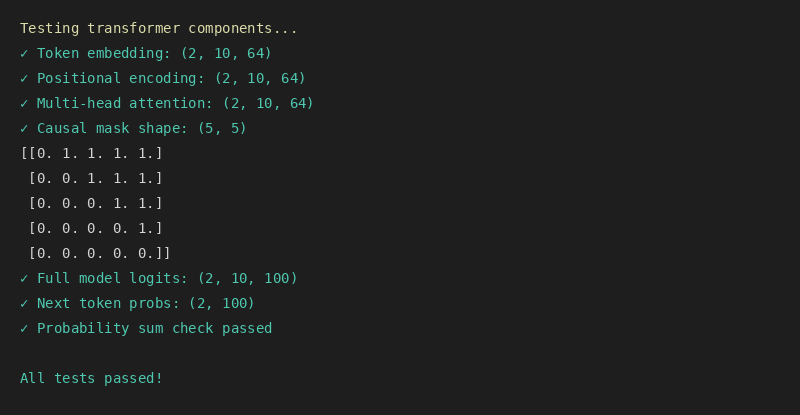
\includegraphics[width=0.9\textwidth]{test_screenshot.png}
\end{center}

Secara keseluruhan, implementasi decoder-only Transformer menggunakan NumPy telah berhasil direalisasikan dengan semua komponen bekerja sesuai spesifikasi matematis. Source code lengkap dapat diakses di: \url{https://github.com/iZcy/transformer-numpy}

\end{document}
